\subsection{Login / Register Page (Interface Mockup)}

\begin{figure}[h!]
\centering
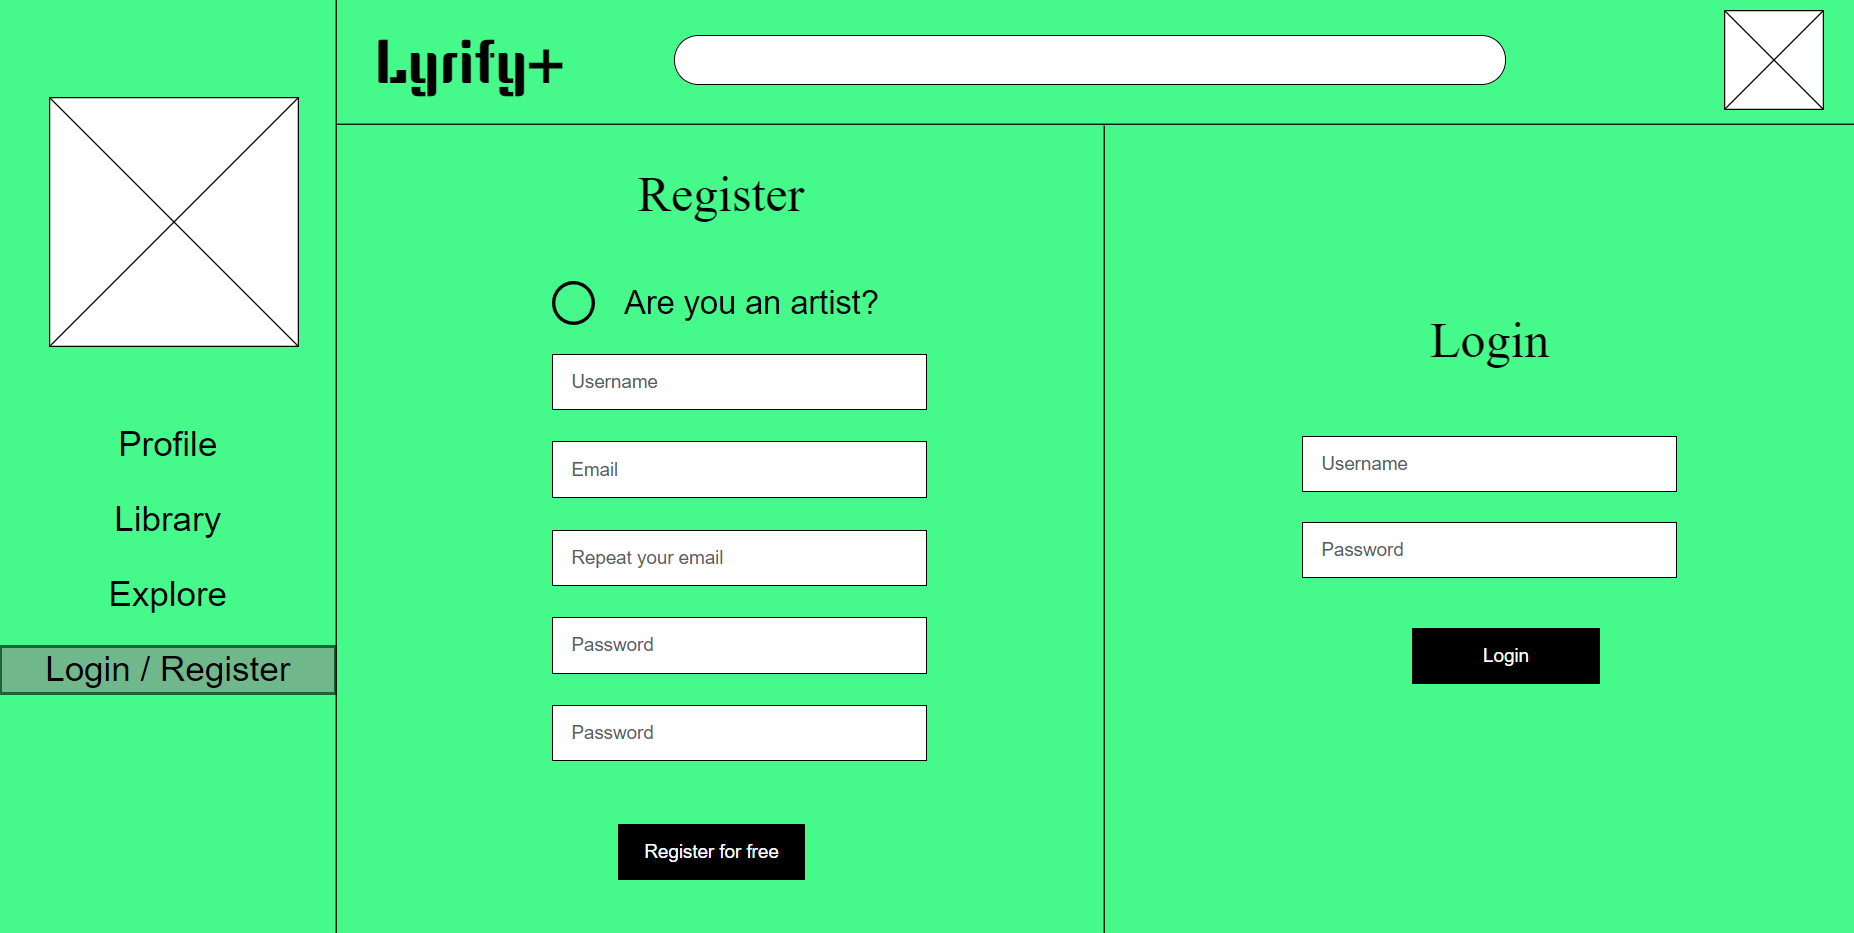
\includegraphics[width=0.9\textwidth]{sections/PLL/LoginPageMockup.png}
\caption{Login page}
\end{figure}

The Login/Register page is the first page that appears when accessing Lyrify+ on the browser. Here, the user can either register as a new user or artist or login if they already have an account. 
For the register form, the user will be asked to: mark the radial button in case he wants to create an account as an artist, enter an username, an email and confirm it and a password also with its confirmation. The username to be provided can have as much as 50 characters, the email is required to have the typical email schema and the password will be required to be between 8 to 25 characters. By clicking the 'Register for free' button the user's credentials will be added to our database and the user will be redirected to the homepage, or to the artist profile page in case they registered as an artist.  
For the login form the user is required to enter their credentials (username and password) and then click the 'Login' button that will check if the credentials are correct and if they are in our database. Once completed the users will be redirected to the homepage and the artists will be redirected to the artist profile page.